Building on Chapter \ref{chap:nts} which verified Moltres' neutronics modeling
capabilities in the context of the \gls{MSFR}, this chapter will cover the
steady-state multiphysics simulation results of the \gls{MSFR} using Moltres.
The steady-state results depend heavily on both neutronics and
thermal-hydraulics solving capabilities in Moltres. Thus, this exercise is the
first verification step for Moltres as a multiphysics \gls{MSR} simulation
tool. This chapter will specifically discuss the temperature, velocity,
neutron flux, and precursor distributions and compare them with data from the
literature. The steady-state operating conditions will also serve as the
initial conditions for the subsequent accident transient simulations.

This chapter will first
present a summary of the procedure for obtaining the steady-state results.
Next, the chapter discusses the steady-state results without modeling decay
heat in direct comparison with the steady-state results from the Polimi and
TUDelft models \cite{aufiero_development_2014}. After this
comparison, the chapter separately discusses the minor differences in the
results from decay heat modeling in the last subsection.

\section{Simulation Procedure}

The procedure for obtaining the results for the steady-state operating
conditions involved several steps
due to the tightly coupled \glspl{PDE}. First, a preliminary transient
simulation of fluid flow in the \gls{MSFR} core was run, starting from zero
inlet velocity and gradually ramping up to match the nominal flow rate (4.5
m$^3$ s$^{-1}$); otherwise Moltres had difficulty converging to the desired
fully developed flow profile.
Next, these fully developed flow values were imported as initial values for
velocity in the full time-dependent simulation modeling the full coupled
neutronics and thermal-hydraulics multiphysics model. The initial values for
the temperature and neutron group flux distributions are 953 K and
$1 \times 10^{14}$ cm$^{-2}$ s$^{-1}$ uniformly throughout the geometry.
Finally, this work assumes that steady state is reached when the volume
integral values of every variable remain constant (up to 6 significant
figures) for at least four seconds in the simulation; this
time period corresponds to the nominal circulation time of the \gls{MSFR}.

\section{Steady-State Thermal-Hydraulics Results} \label{sec:ss-th}

Figure \ref{fig:flow-temp} shows the temperature and velocity fields of the
fuel salt in the core at steady state from Moltres and the Polimi and TUDelft
models. Figure \ref{fig:flow} provides an alternate view of the flow profile
through flow streamlines superimposed on the velocity magnitude distribution.
The results from Moltres show good qualitative agreement with the Polimi and
TUDelft models \cite{fiorina_modelling_2014}; the plots show similar
flow and hotspot features in all three models. Furthermore, the highest salt
velocities in all three models occur at the inlet, outlet, and at core
half-height approximately 0.40 m away from the central axis. A large
recirculation region forms near the blanket tank walls from turbulent flow.
Inertial forces dominate over viscous forces to form this large eddy. The main
difference between Moltres, and the Polimi and TUDelft models is the flow
profile near the central axis at the top and bottom of the core.
The Polimi and TUDelft models predict relatively stagnant flow in these
regions without recirculation. Moltres, on the other hand, predicts explicit
recirculating flow in these regions. This is due to our constant turbulent
viscosity approximation in Moltres. The k-$\epsilon$ turbulence models in the
Polimi and TUDelft models predict that the turbulent viscosity in these
regions is as high as 100 Pa$\cdot$s, much higher than our 40 Pa$\cdot$s
approximation.

\begin{figure}[htbp!]
    \centering
    \begin{subfigure}[t]{.35\textwidth}
        \centering
        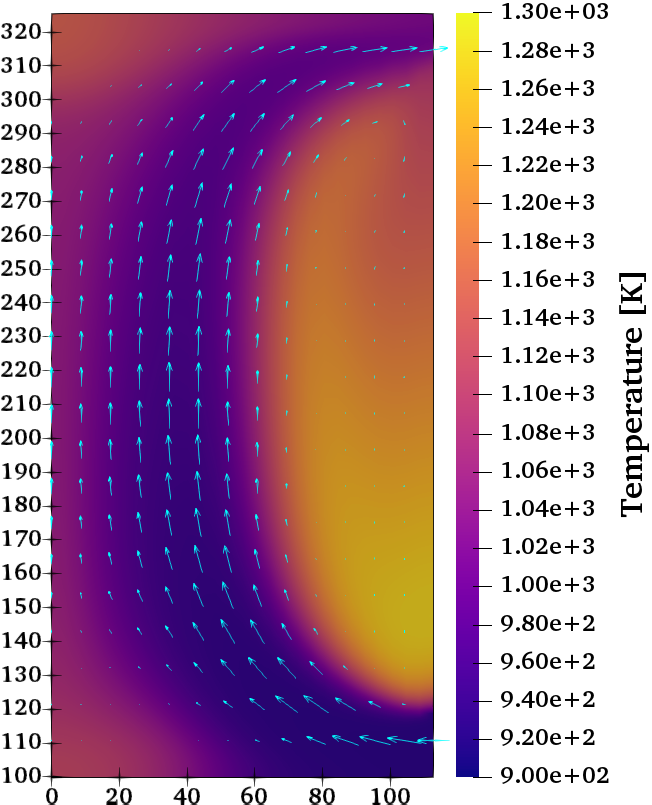
\includegraphics[width=\textwidth]{flow-temp-plasma}
    \end{subfigure}
    \hfill
    \begin{subfigure}[t]{.625\textwidth}
        \centering
        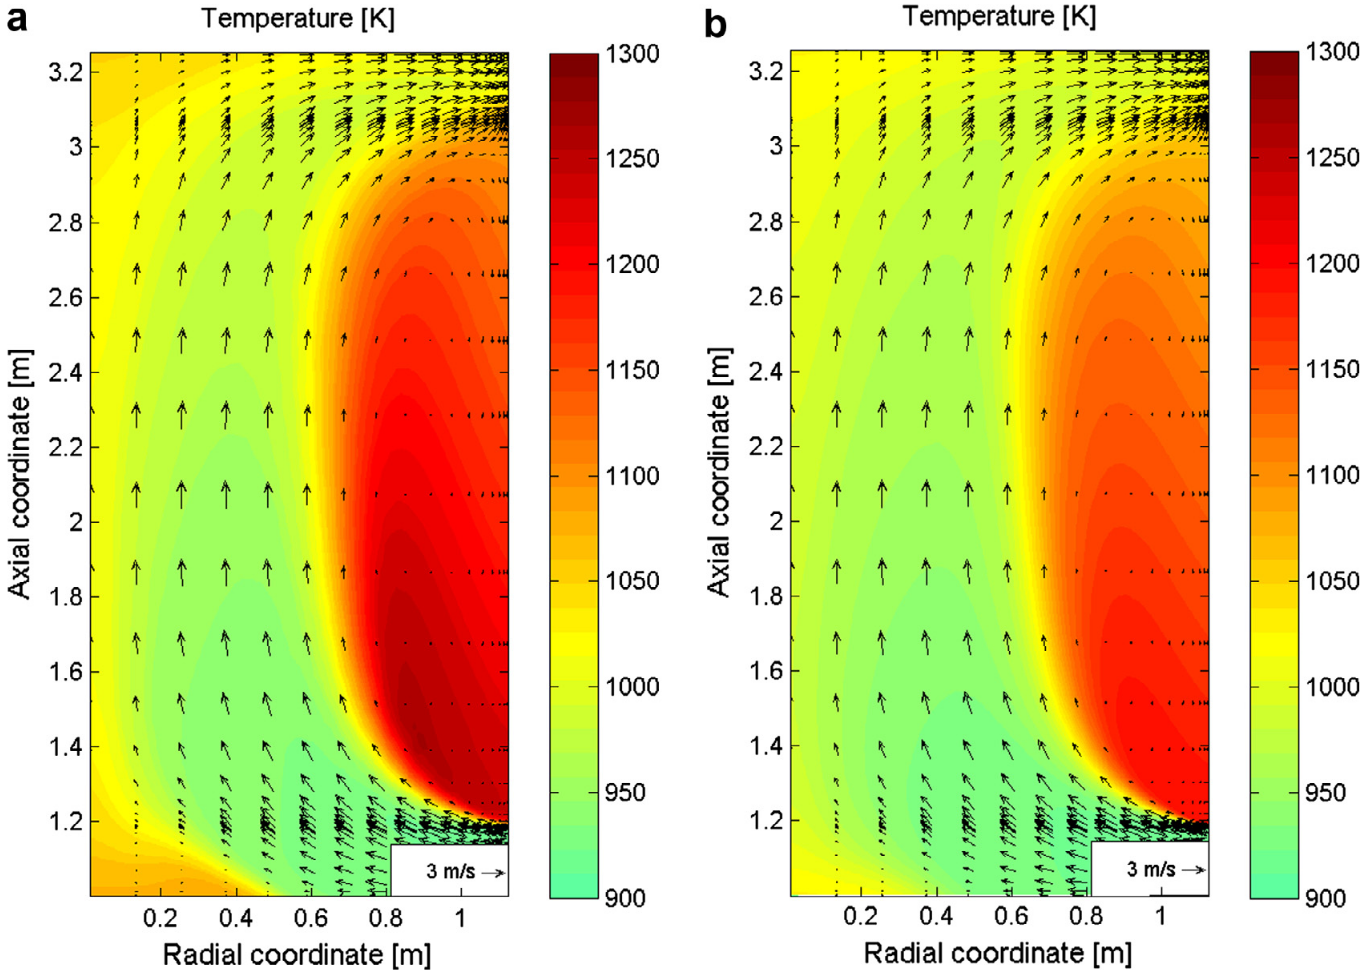
\includegraphics[width=\textwidth]{flow-temp-fiorina}
    \end{subfigure}
    \caption{Temperature and velocity fields in the core from Moltres
    (left), Polimi (center), and TUDelft (right) models. The colors represent
    temperature according to the respective color bars and the arrows
    represent velocity fields.}
    \label{fig:flow-temp}
\end{figure}

\begin{figure}[htbp!]
    \centering
    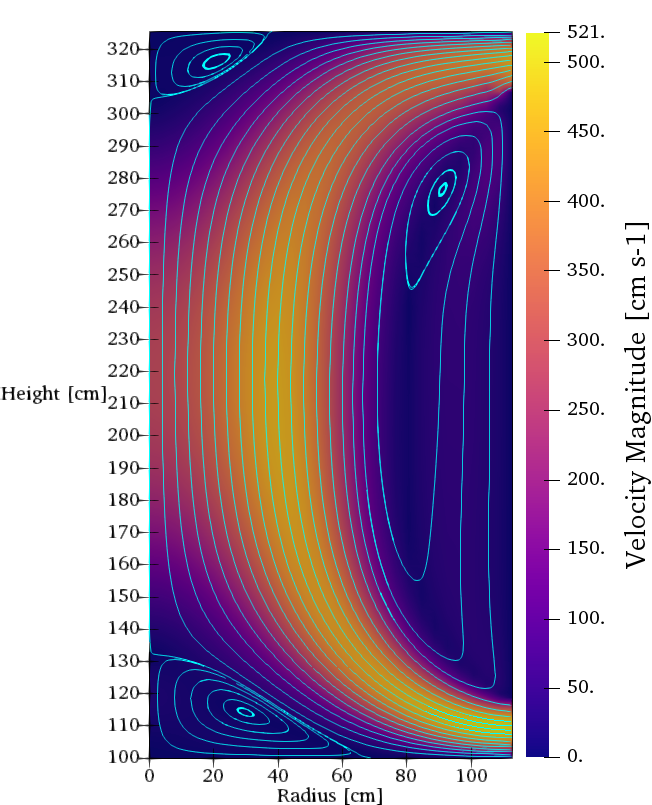
\includegraphics[width=.58\textwidth]{flow-plasma}
    \caption{Fuel salt flow streamlines and velocity magnitude in the core.
    The colors represent velocity magnitude according to the color bar on the
    right.}
    \label{fig:flow}
\end{figure}

Nevertheless, similar temperature hotspots form in these regions of
recirculation and stagnation as convection is the dominant heat transfer
mechanism. The maximum temperature from Moltres, 1275 K near the bottom of the
large recirculation zone, is closer to the maximum temperature in the Polimi
model ($\approx$ 1300 K) than the TUDelft model ($\approx$ 1200K). Similarly,
the plots show cooler temperatures in high-velocity regions. The minimum
temperature is 924 K at the inlet. 

Although the temperatures at the hotspots are well below the melting point of the Ni-alloy structure (1500 K), they may cause undue thermal stress on the
blanket tank structure and accelerate salt corrosion rates. A
sudden, large reactivity insertion could push fuel salt temperatures above the
melting point of the Ni-alloy and cause irreversible damage. Furthermore,
the reservoir of hot fuel salt may cause unpredictable behavior during
transient scenarios when the flow profile fluctuates.
Thus, Rouch et al. \cite{rouch_preliminary_2014} developed an improved
hourglass-shaped design for the central core region to optimize flow
distribution and prevent these
recirculation zones and hotspots from forming. A study of this new design
using Moltres is a potential subject for future work when a proper turbulence
model is in place.

\section{Steady-State Neutronics Results}

\subsection{Neutron Flux}

The neutron flux distribution represents the heat source distribution in a
nuclear reactor. Figure \ref{fig:neutronflux} shows the neutron flux
distributions in the core for all six neutron energy groups, and Figure
\ref{fig:axialradial} shows the axial and radial fluxes along the center of
the core and at reactor half-height, respectively.
The distributions are highly symmetric along the
central and horizontal axes, as expected of a cylindrical reactor design. The
lower temperatures near the center of the core promote the neutron
flux peaking but it is of little concern as no neutronically vulnerable
structures exist in that region. The peak total flux at the center is
$9.80 \times 10^{15}$ cm$^{-2}\cdot$s$^{-1}$, which is close to values
reported by Fiorina et al. \cite{fiorina_molten_2013} and Aufiero et al.
\cite{aufiero_development_2014} as shown in Table \ref{table:peak-flux}. The
peak flux value from this paper is slightly higher as this work used the
heterogeneous temperature distribution in Figure \ref{fig:flow-temp} while
Fiorina et al. and Aufiero et al. imposed uniform temperature distributions
at 973 K.

\begin{figure}[b!]
    \centering
    \begin{subfigure}[t]{.325\textwidth}
        \centering
        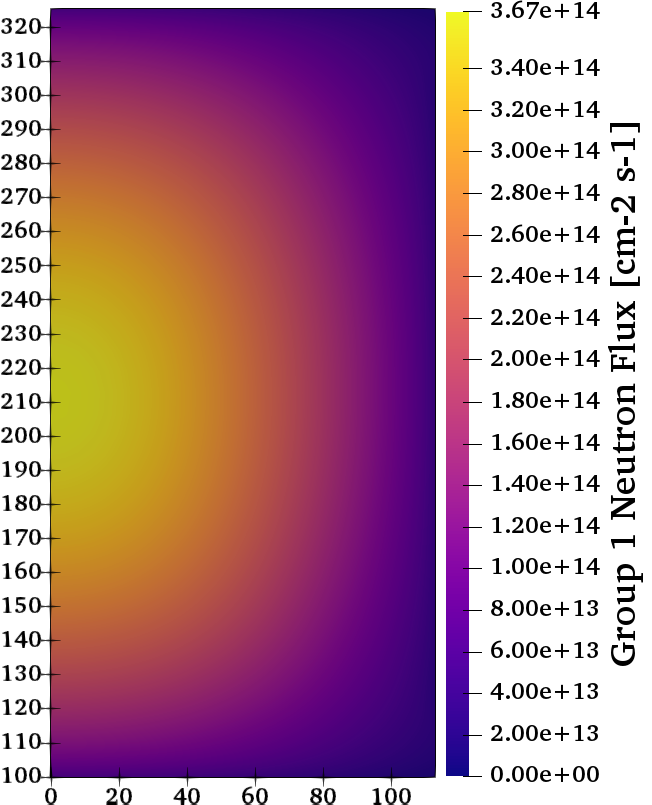
\includegraphics[width=\textwidth]{g1}
    \end{subfigure}
    \begin{subfigure}[t]{.325\textwidth}
        \centering
        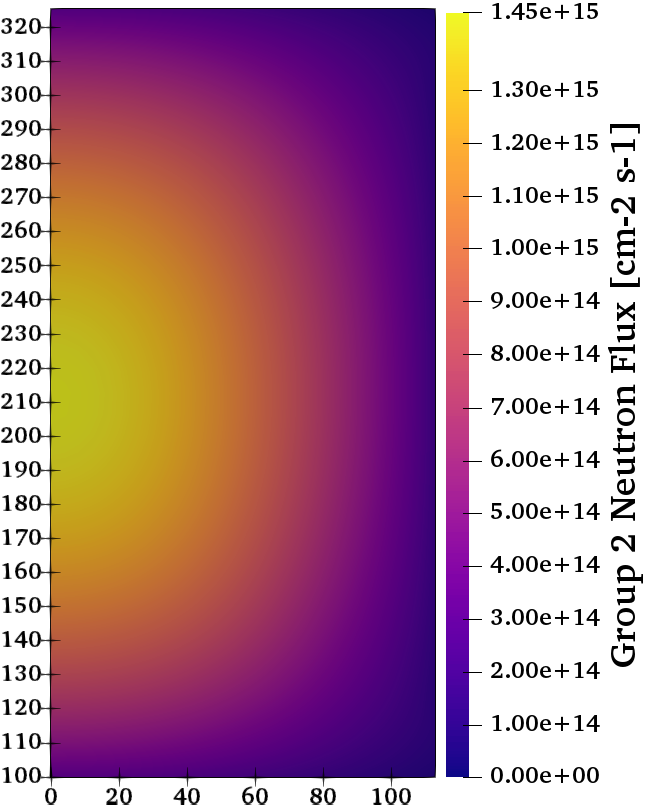
\includegraphics[width=\textwidth]{g2}
    \end{subfigure}
    \begin{subfigure}[t]{.325\textwidth}
        \centering
        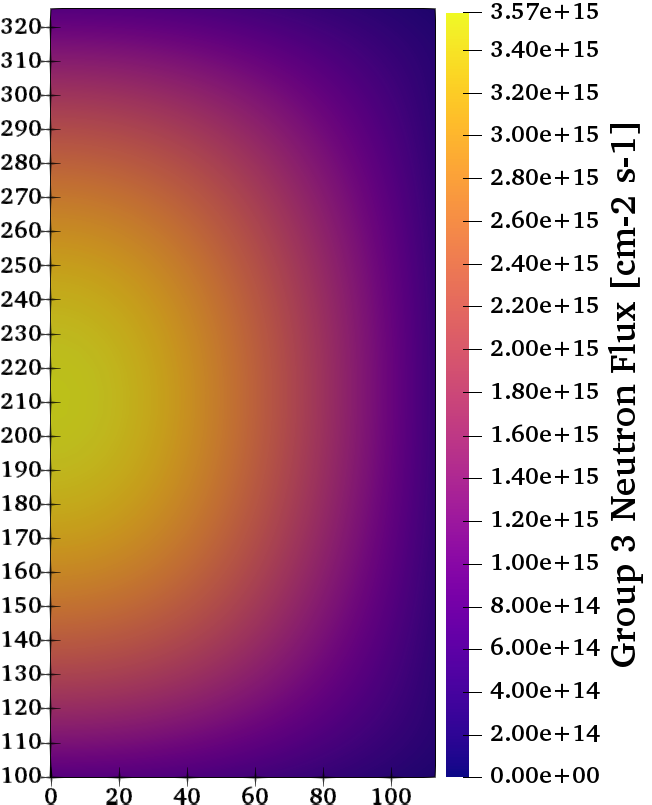
\includegraphics[width=\textwidth]{g3}
    \end{subfigure}
    \begin{subfigure}[t]{.325\textwidth}
        \centering
        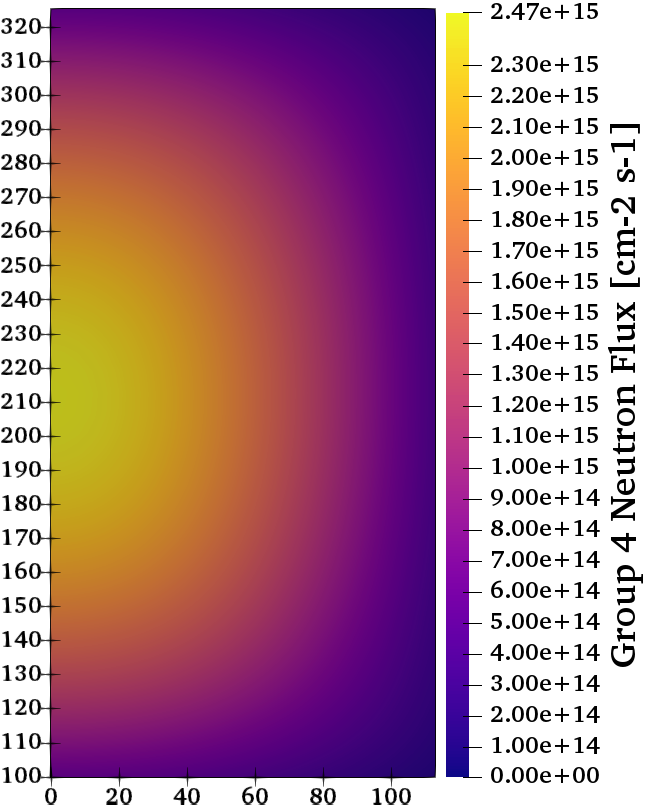
\includegraphics[width=\textwidth]{g4}
    \end{subfigure}
    \begin{subfigure}[t]{.325\textwidth}
        \centering
        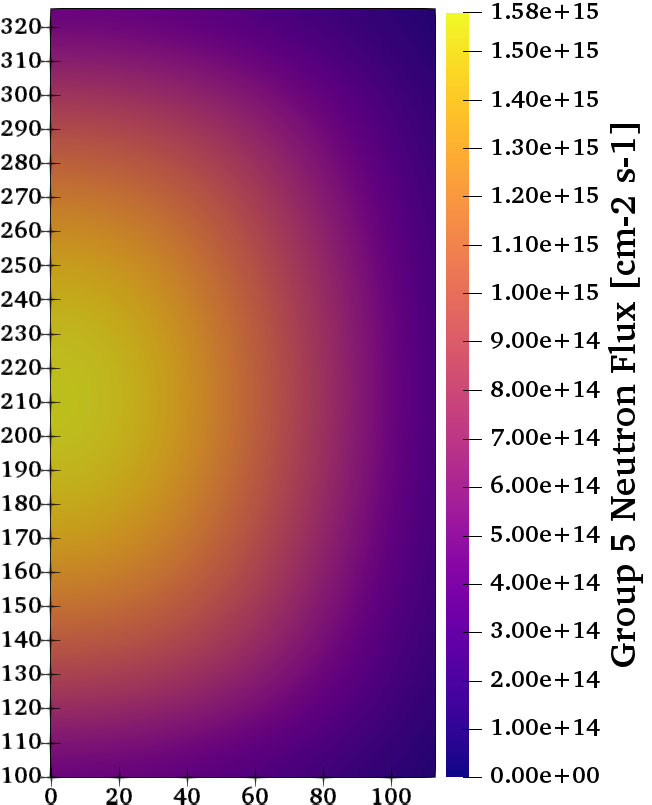
\includegraphics[width=\textwidth]{g5}
    \end{subfigure}
    \begin{subfigure}[t]{.325\textwidth}
        \centering
        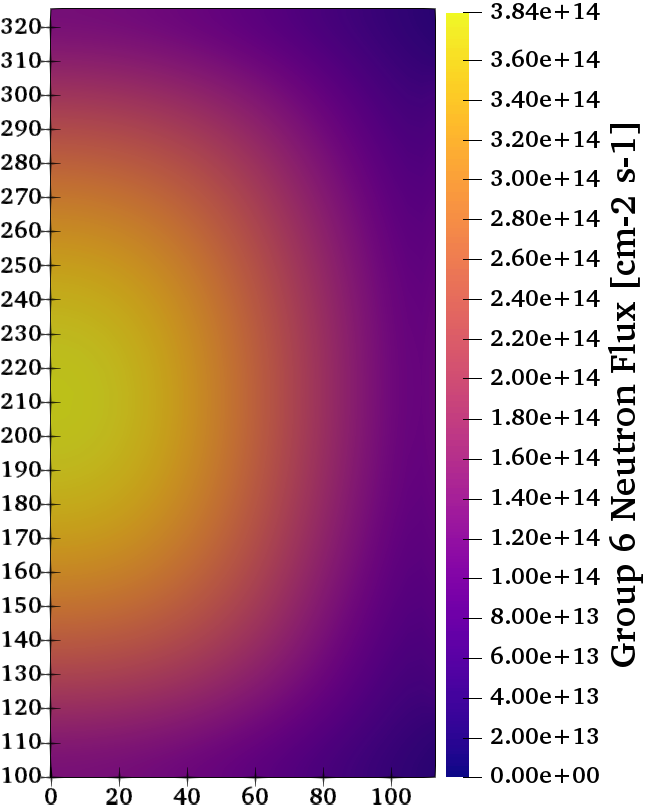
\includegraphics[width=\textwidth]{g6}
    \end{subfigure}
    \caption{Neutron flux distributions in the core for neutron energy groups
    1 to 6. The y and x axes represent height and radius (in cm) of the core
    relative to the entire reactor geometry.}
    \label{fig:neutronflux}
\end{figure}

\begin{figure}[t!]
    \centering
    \begin{subfigure}[t]{.49\textwidth}
        \centering
        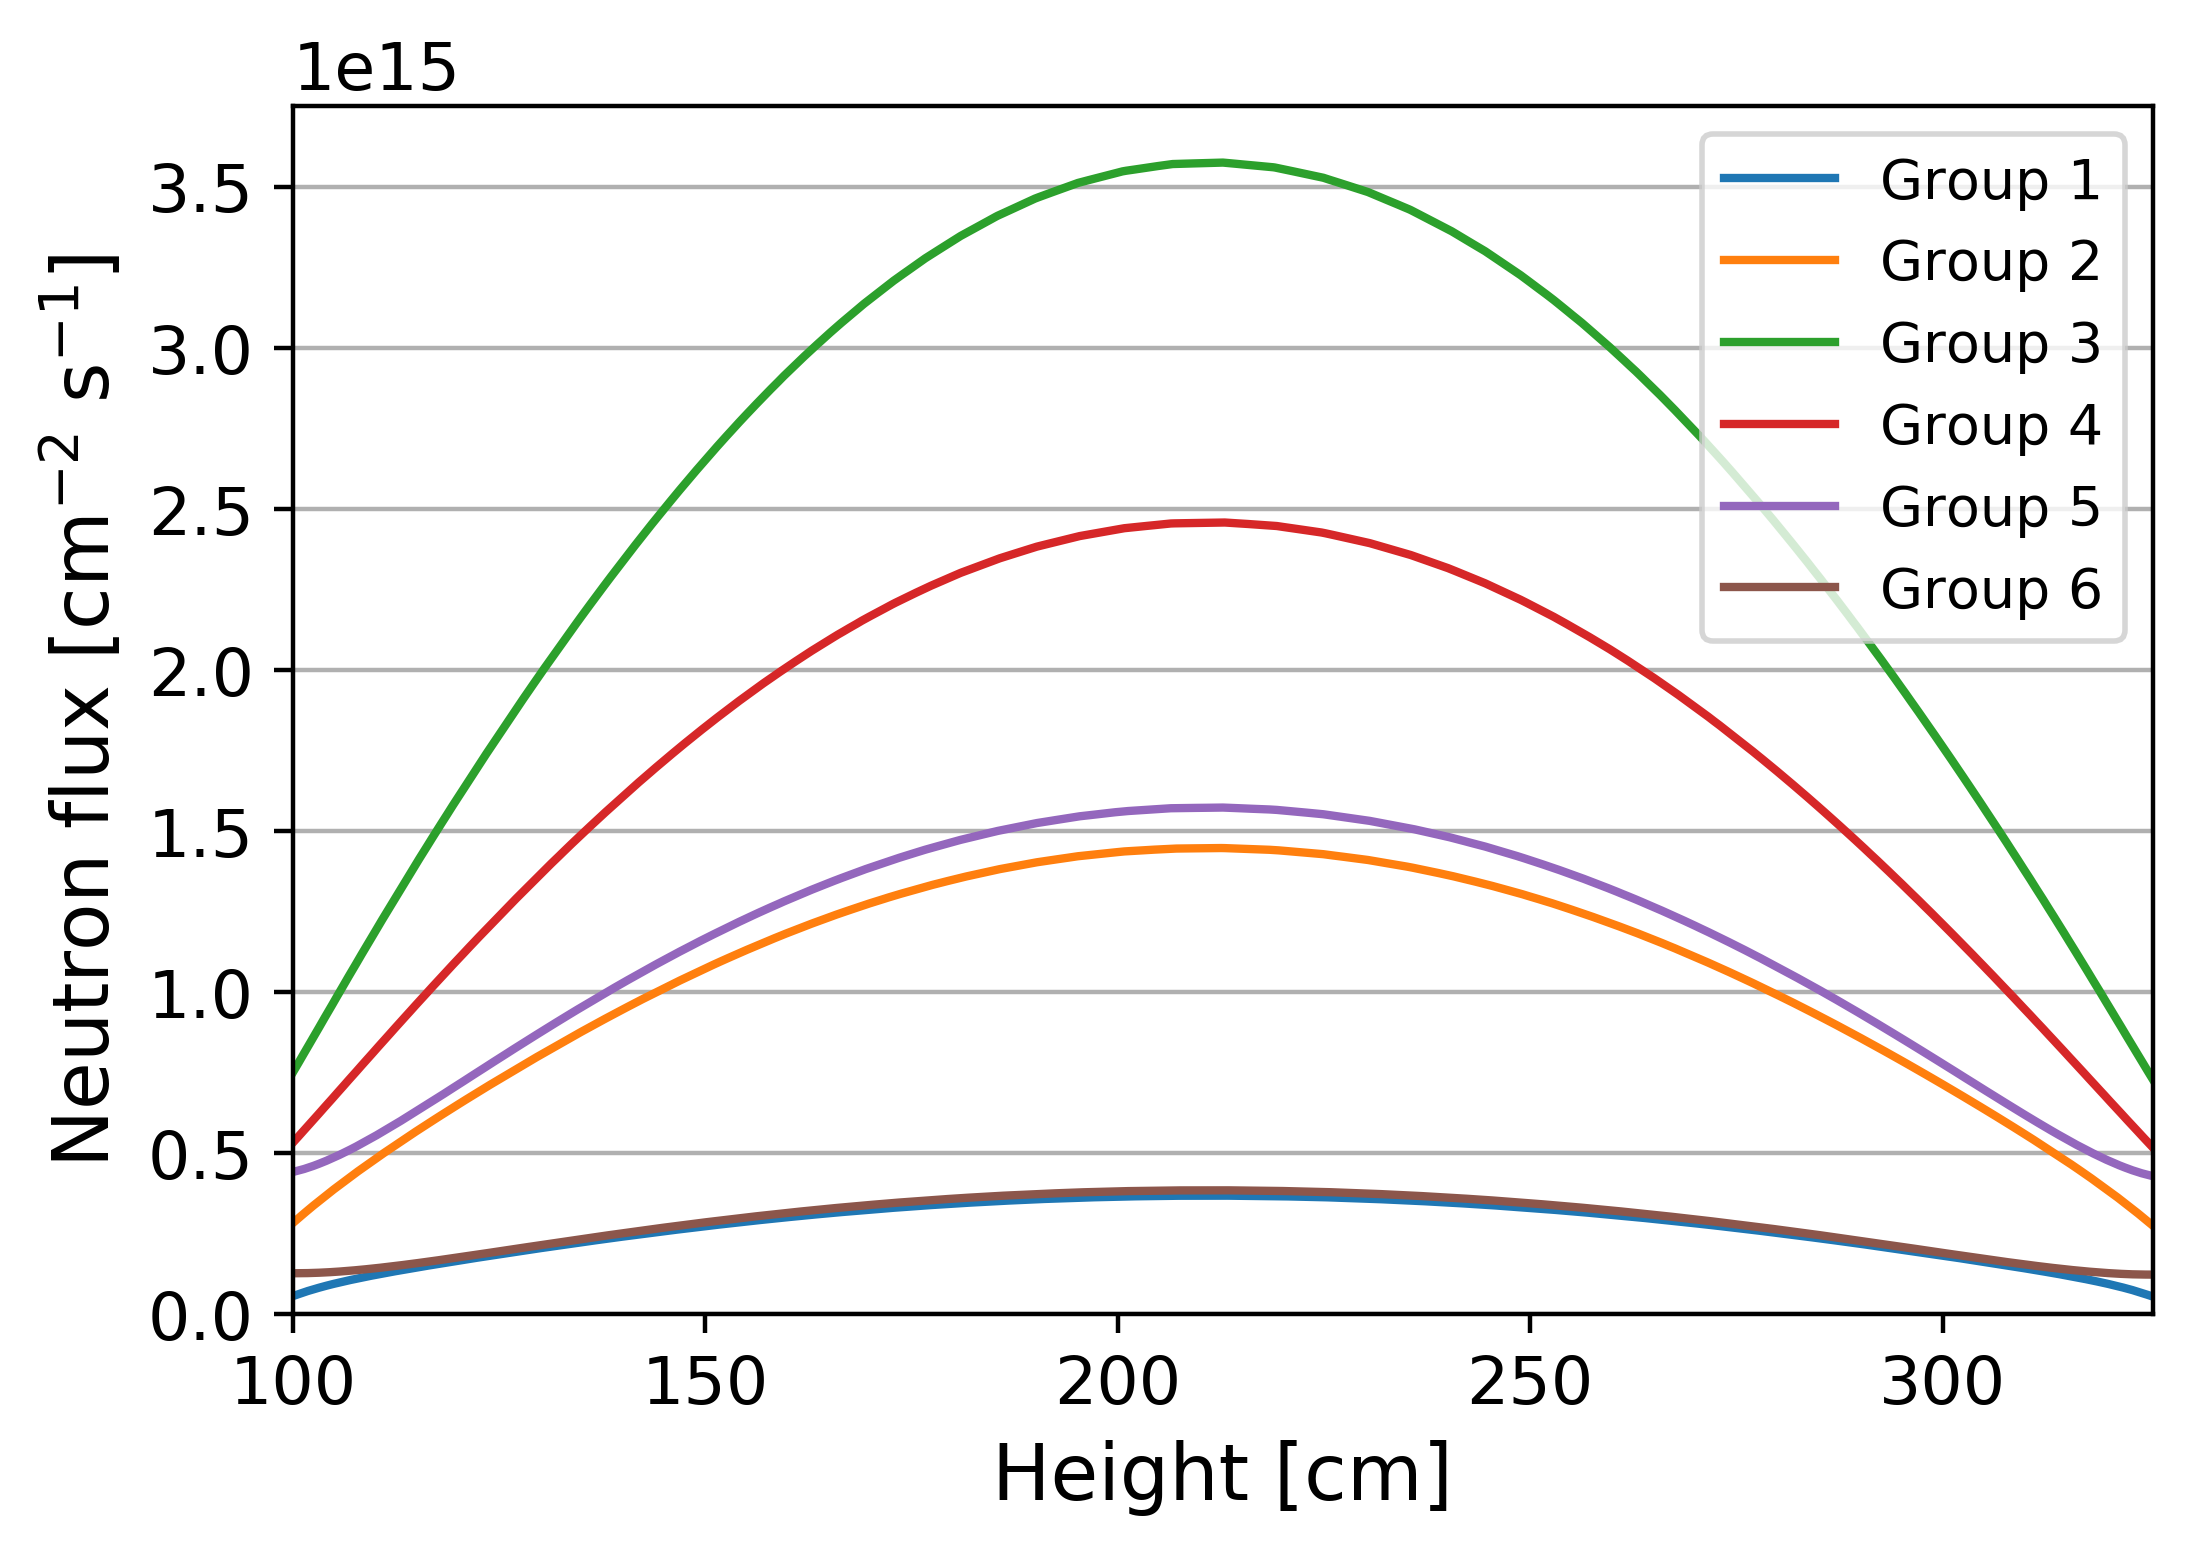
\includegraphics[width=\textwidth]{axial-flux}
    \end{subfigure}
    \begin{subfigure}[t]{.49\textwidth}
        \centering
        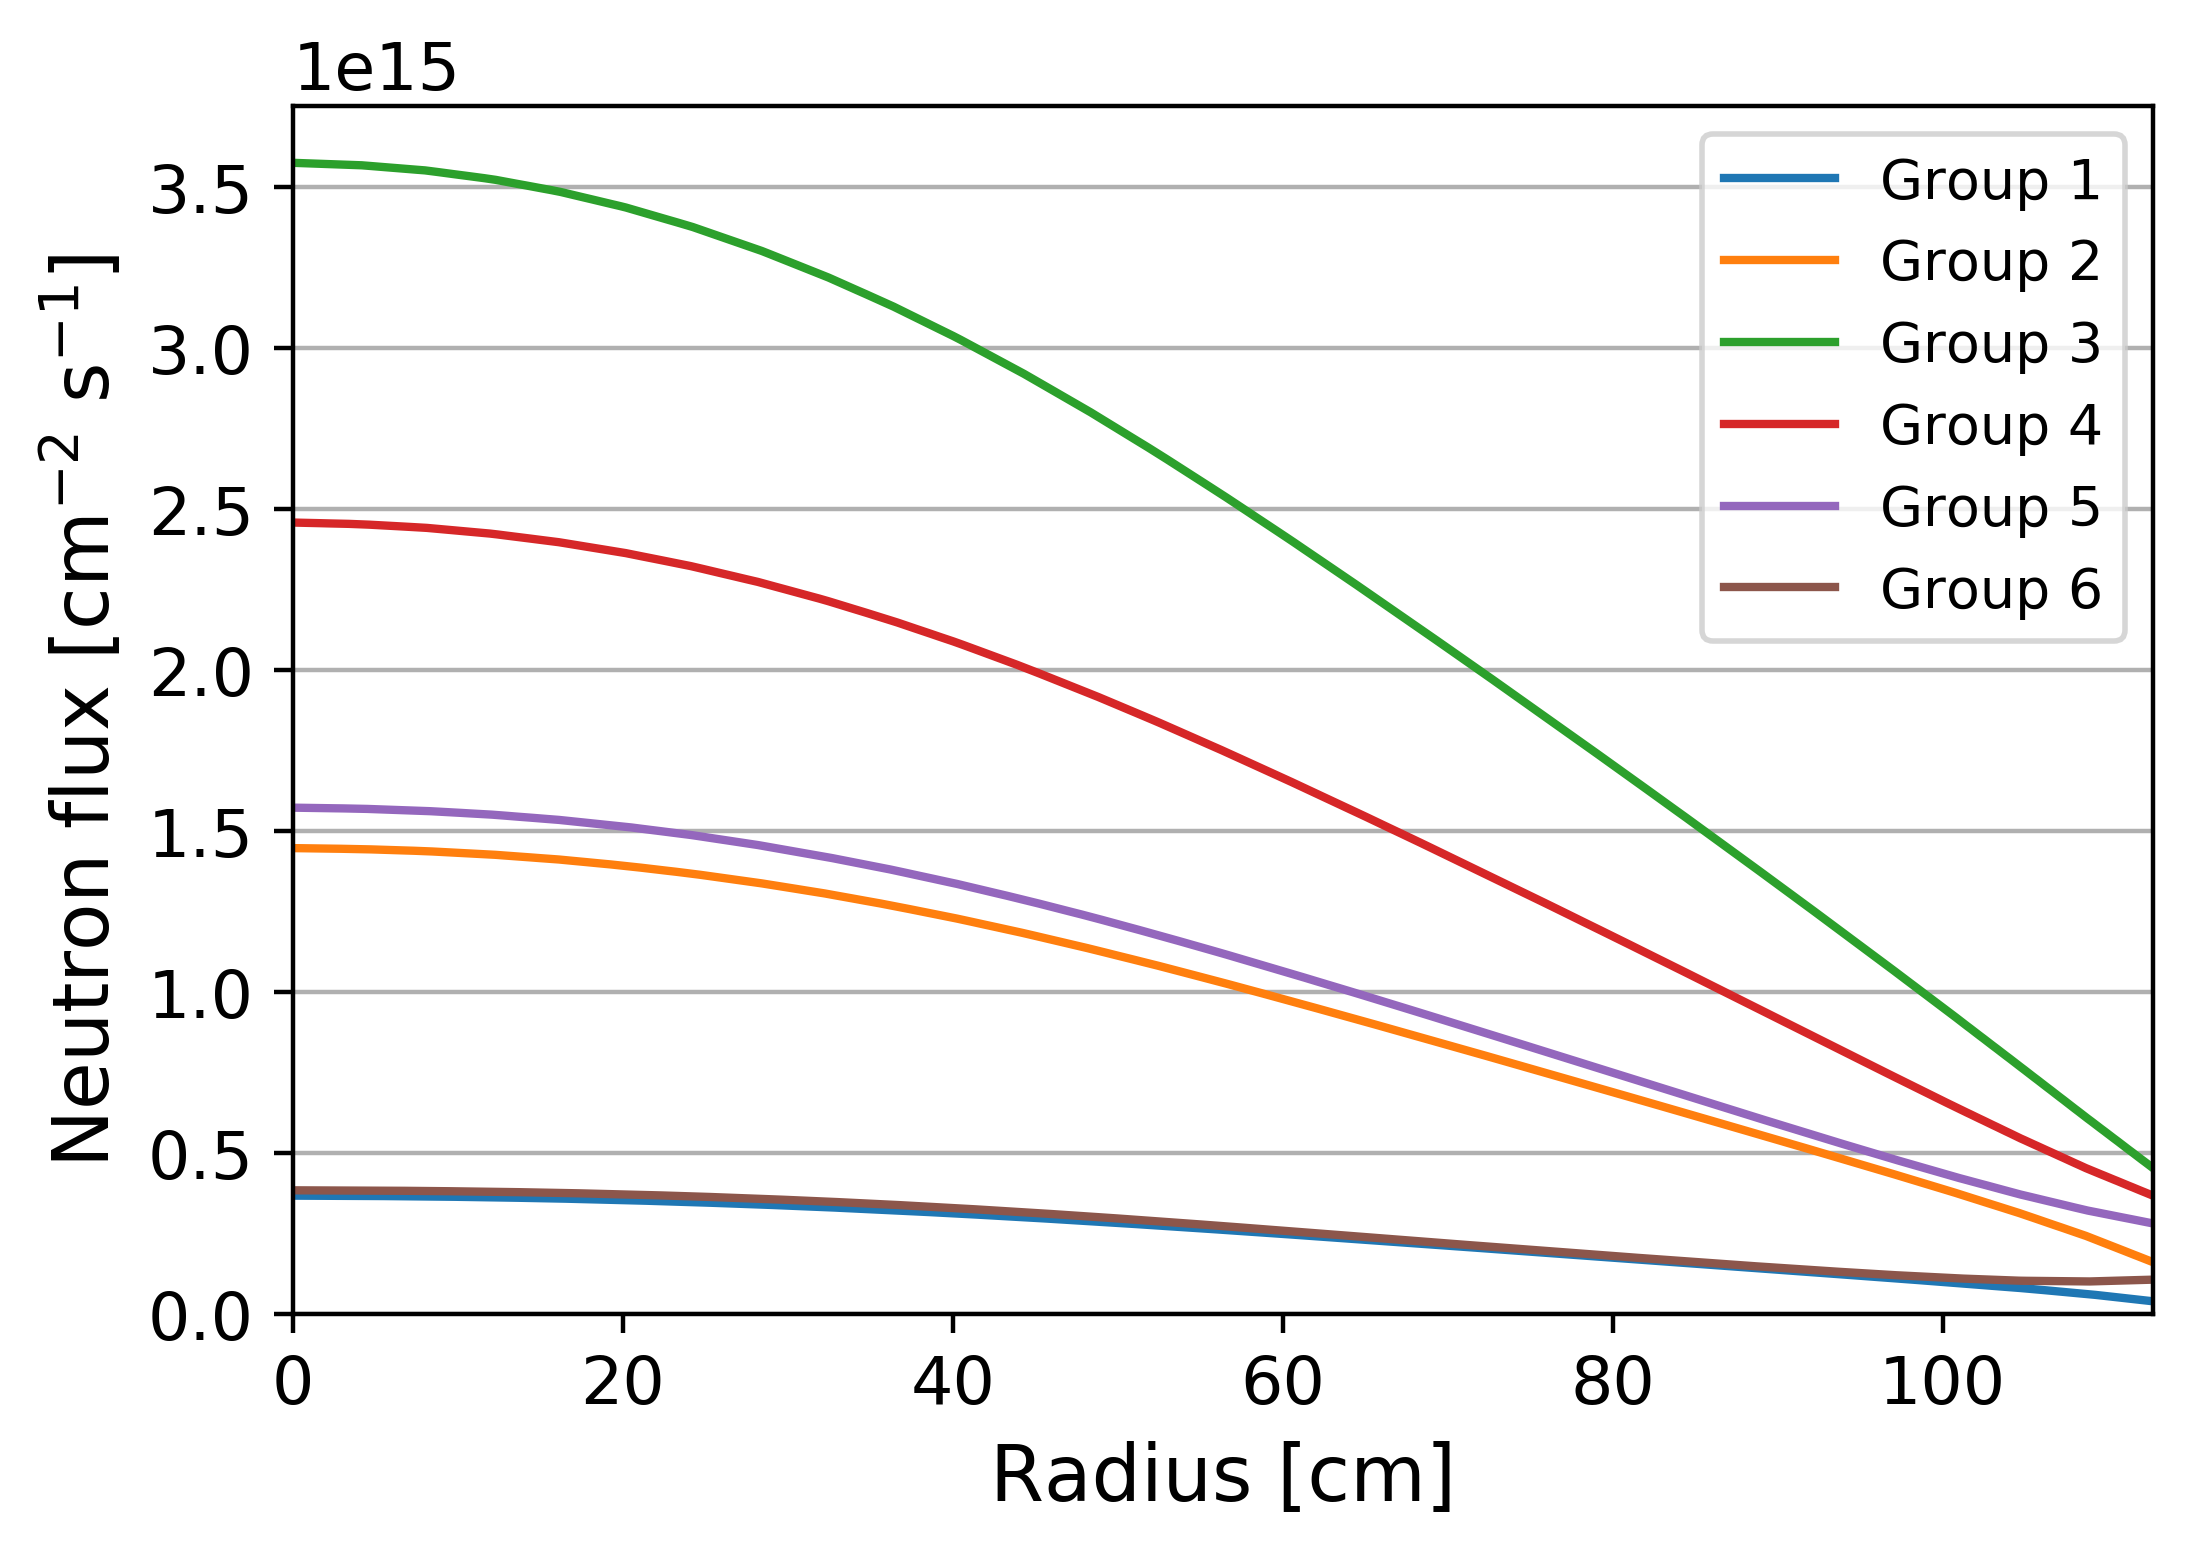
\includegraphics[width=\textwidth]{radial-flux}
    \end{subfigure}
    \caption{Axial (left) and radial (right) neutron flux distributions in the
    core for neutron energy groups 1 to 6.}
    \label{fig:axialradial}
\end{figure}

\begin{table}[b!]
	\centering
	\caption{Peak neutron flux values from Moltres (this paper), COMSOL
	\cite{fiorina_molten_2013}, and OpenFOAM \cite{aufiero_development_2014}
	models along with the temperature distribution with which the values were
	obtained.}
	\begin{tabular}{l l S}
		\toprule
		{Model} & {Temperature distribution} & {Peak Neutron Flux [$\times 10^{15}$ cm$^{-2}$ s$^{-1}$]}
		\\
		\midrule
		{Moltres (This paper)} & {Steady state} & 9.80\\
		{COMSOL} & {Uniform, 973 K} & 8.6 \\
		{OpenFOAM} & {Uniform, 973 K} & 9.0 \\
		\bottomrule
	\end{tabular}
	\label{table:peak-flux}
\end{table}

\begin{figure}[t!]
    \centering
    \begin{subfigure}[t]{.243\textwidth}
        \centering
        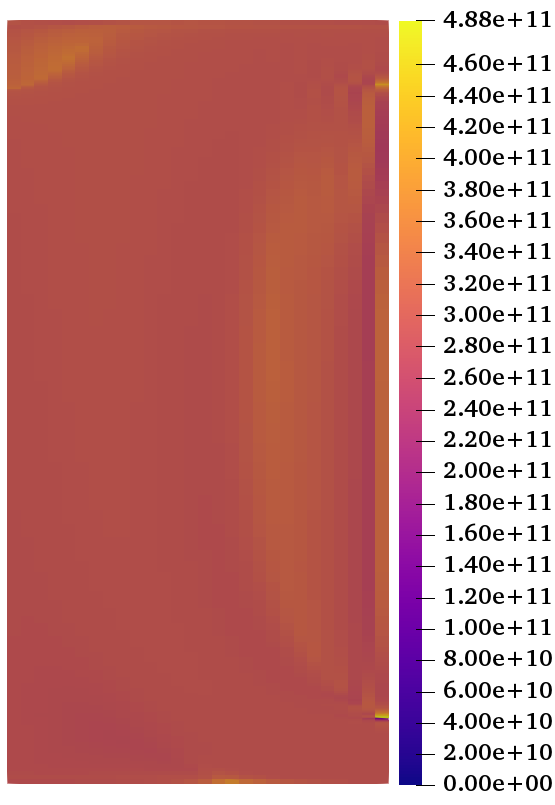
\includegraphics[width=\textwidth]{pre1}
    \end{subfigure}
    \begin{subfigure}[t]{.243\textwidth}
        \centering
        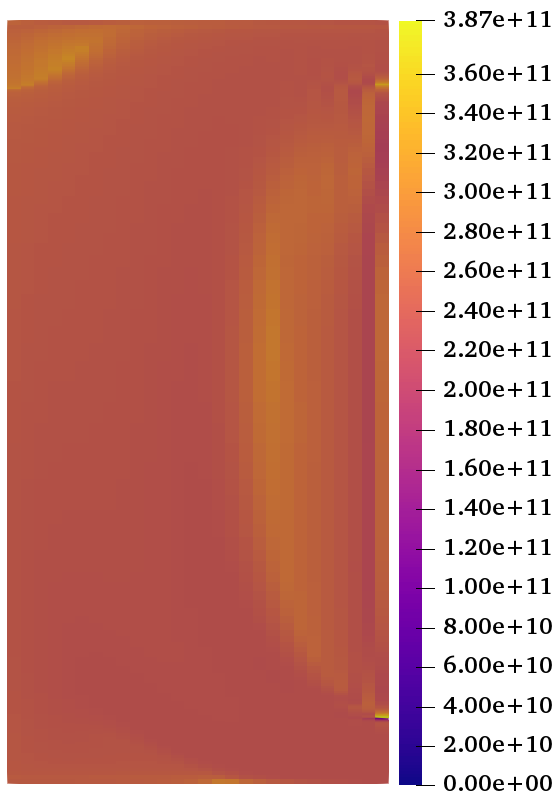
\includegraphics[width=\textwidth]{pre2}
    \end{subfigure}
    \begin{subfigure}[t]{.243\textwidth}
        \centering
        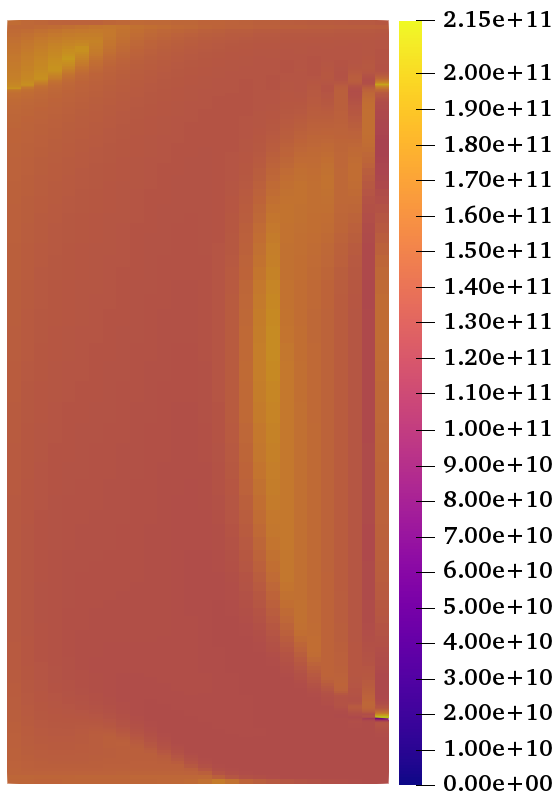
\includegraphics[width=\textwidth]{pre3}
    \end{subfigure}
    \begin{subfigure}[t]{.243\textwidth}
        \centering
        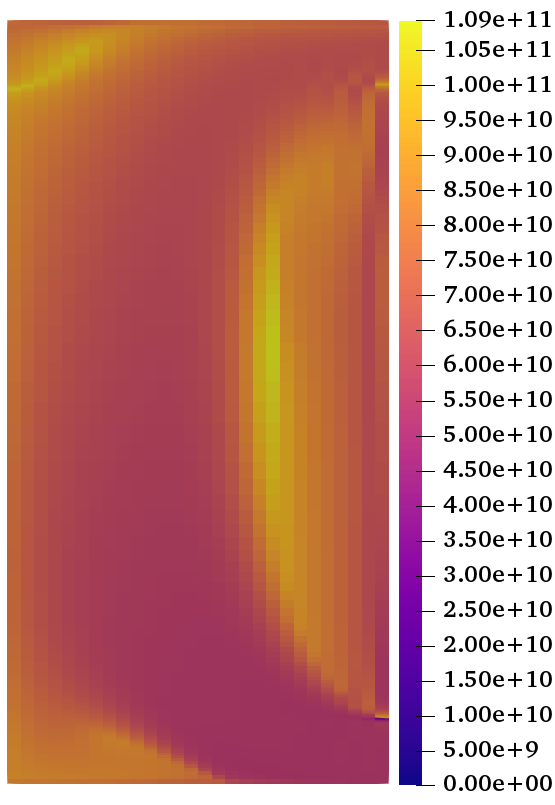
\includegraphics[width=\textwidth]{pre4}
    \end{subfigure}
    \begin{subfigure}[t]{.243\textwidth}
        \centering
        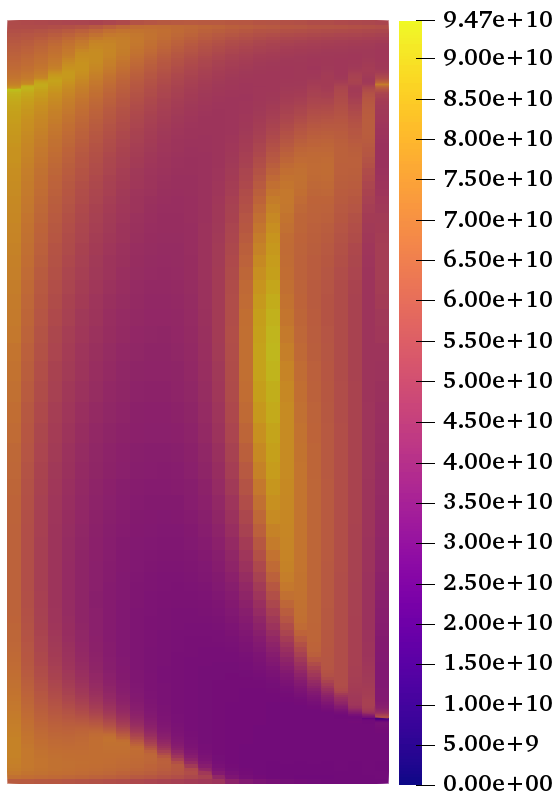
\includegraphics[width=\textwidth]{pre5}
    \end{subfigure}
    \begin{subfigure}[t]{.243\textwidth}
        \centering
        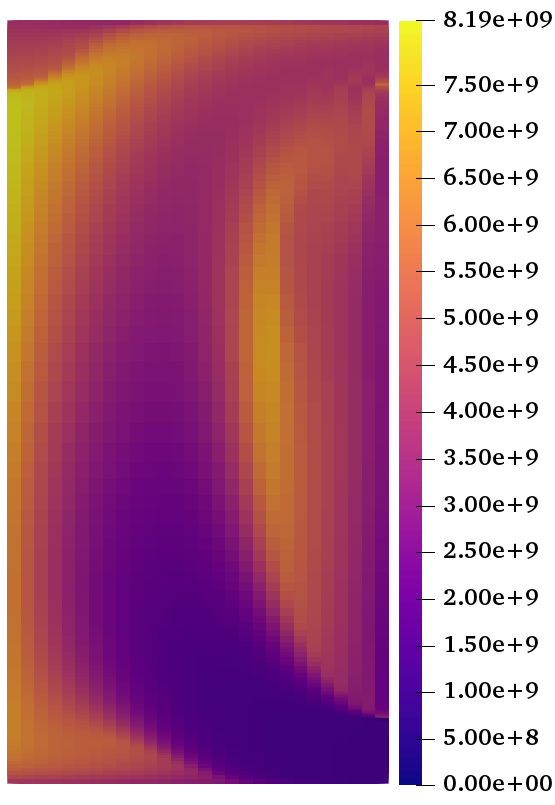
\includegraphics[width=\textwidth]{pre6}
    \end{subfigure}
    \begin{subfigure}[t]{.243\textwidth}
        \centering
        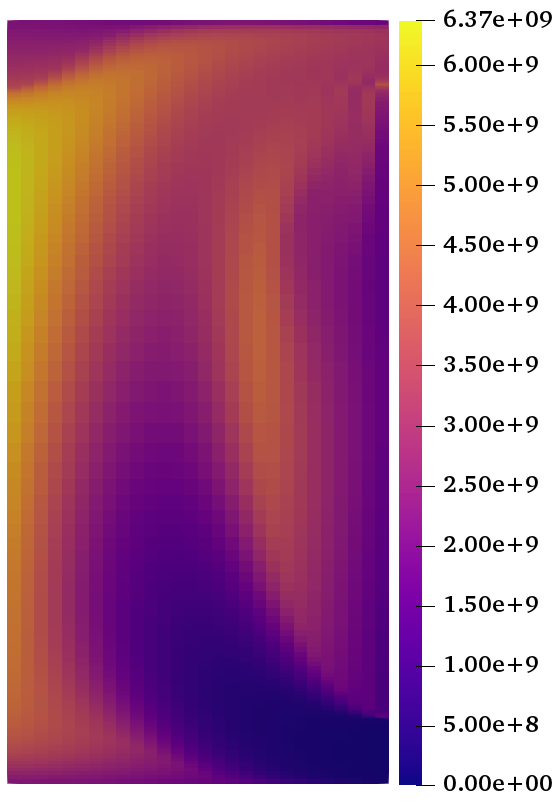
\includegraphics[width=\textwidth]{pre7}
    \end{subfigure}
    \begin{subfigure}[t]{.243\textwidth}
        \centering
        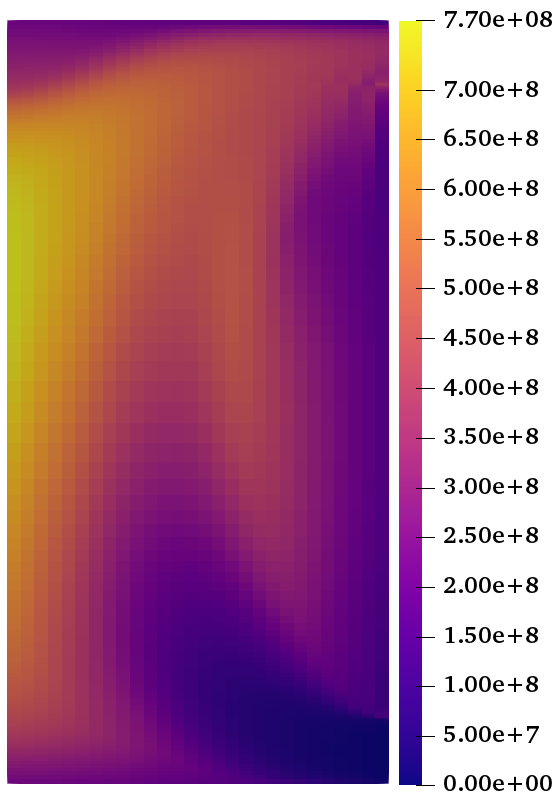
\includegraphics[width=\textwidth]{pre8}
    \end{subfigure}
    \caption{\gls{DNP} distributions in the core for \gls{DNP} groups
    1 to 8 (from left to right, top to bottom). Refer to Figure \ref{fig:neutronflux} for the height and radius
    scales on the y and x axes, respectively. Note the different scales for
    each distribution.}
    \label{fig:dnp}
\end{figure}

\subsection{Delayed Neutron Fraction}

As mentioned earlier, the delayed neutron precursors (DNPs) are mobile in
\glspl{MSR} and their distributions do not directly correspond to the neutron
flux distributions. The location where the \glspl{DNP} decay and emit neutrons
impacts their neutron
importance depending on their proximity to fissile and parasitic isotopes.
Figure \ref{fig:dnp} shows the \gls{DNP} distributions for all eight \gls{DNP}
groups. In general, the figures show less \glspl{DNP} in the regions with fast
salt flow. The
precursors from the shortest-lived group (Group 8) predominantly decay within
the core as their half-lives are shorter than the time it takes to reach the
outlet while the precursors from the longest-lived group (Group 1) are
relatively evenly distributed due to their long half-lives. For the
longer-lived groups, the \gls{DNP} concentrations are ill-resolved on the
mesh elements adjacent to the outlet and the inlet boundaries, respectively.
Thus, the present author recommends careful mesh refinement for future work
involving similar geometries.

\begin{figure}[b!]
    \centering
    \begin{subfigure}[t]{.30\textwidth}
        \centering
        \vspace{.9cm}
        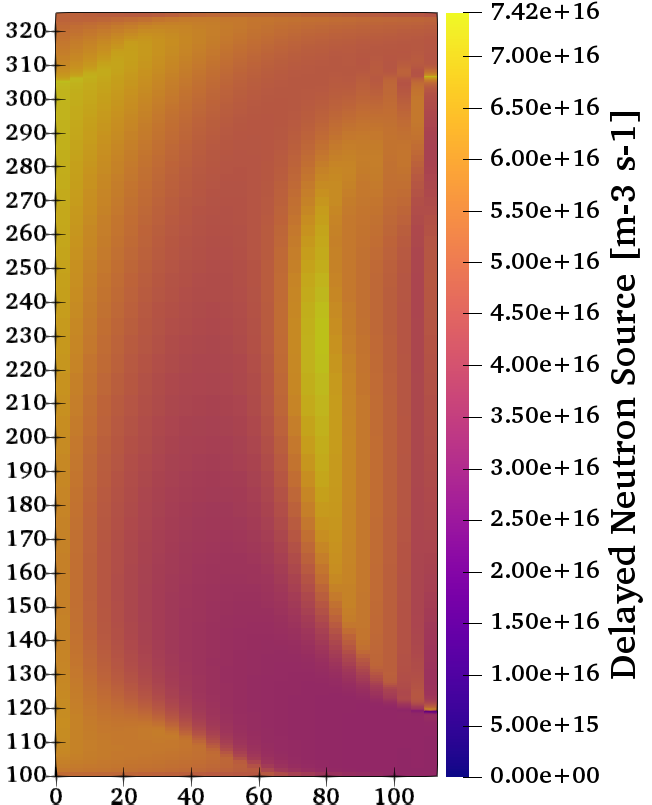
\includegraphics[width=\textwidth]{pre}
    \end{subfigure}
    \begin{subfigure}[t]{.69\textwidth}
        \centering
        \vspace{0pt}
        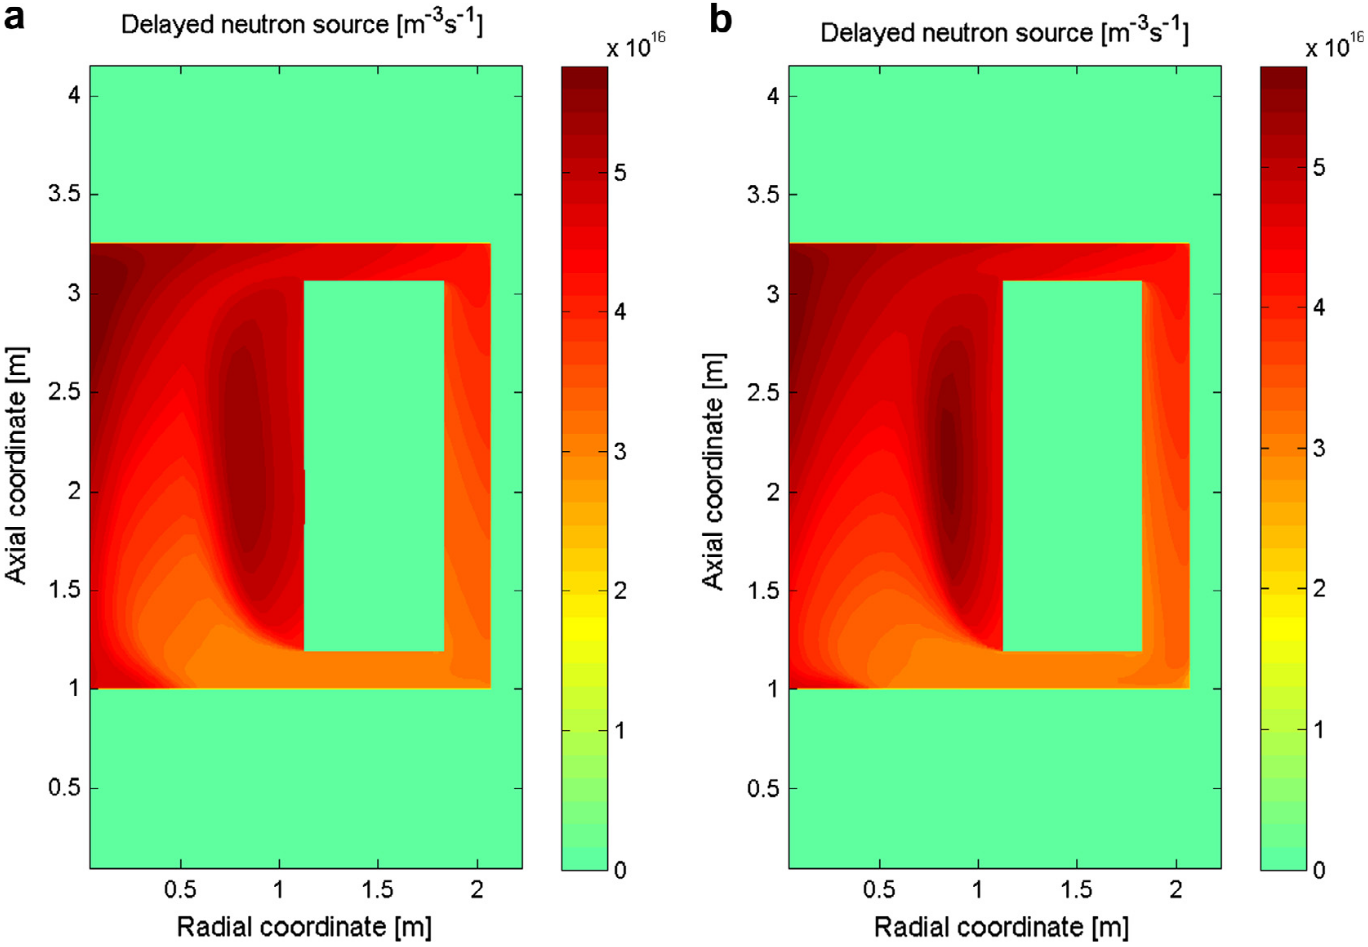
\includegraphics[width=\textwidth]{fiorina-pre}
    \end{subfigure}
    \caption{Total delayed neutron source distribution in the core from
    Moltres (left), Polimi (center), and TUDelft (right) models.}
    \label{fig:pre}
\end{figure}

Figure \ref{fig:pre} compares the total delayed neutron source
distribution from Moltres with the results from the Polimi and TUDelft models
\cite{fiorina_modelling_2014}. In contrast to Figure \ref{fig:dnp} which shows
the precursor distribution, Figure \ref{fig:pre} shows the rate of delayed
neutron emission, which was calculated by multiplying each \gls{DNP} group
$C_i$ with its associated decay constant $\lambda_i$.
The Polimi and TUDelft models
feature greater \gls{DNP} retention in the stagnant regions in the core. This
effect is less pronounced in the Moltres model, most notably at the top of the
core near the central axis and in the recirculation zone adjacent to the
blanket tank. As mentioned in Section \ref{sec:ss-th}, only the Moltres model
features a small recirculation zone at the top of the core. This local flow
pattern is responsible for diverting the shorter-lived \glspl{DNP} away from
the top of the core and reducing the build-up in that region.

The in-core delayed neutron fraction, which we denote as $\beta_c$, is an
important safety parameter for \glspl{MSR}. This value represents the actual
delayed neutron fraction in \glspl{MSR} after accounting for the loss of
delayed neutrons from \glspl{DNP} decaying outside the active core region.
Reactors with smaller $\beta$ values exhibit greater prompt jumps in the
neutron flux in response to reactivity insertions because they have a greater
proportion of prompt neutrons under normal operating conditions. This is
undesirable from a reactor safety perspective because it reduces the time
available for active safety mechanisms to
activate and scram the reactor. In \glspl{MSR}, this danger is partly
mitigated by the strong, negative fuel temperature reactivity coefficient. 
Chapter 6 contains more in-depth discussions for various transient scenarios.

Table \ref{table:dnf} compares the fraction of out-of-core emissions and
the $\beta_c$ values from Moltres with the Polimi and TUDelft models. The
present author calculated the fraction of out-of-core emissions by finding the
average concentration of each \gls{DNP} group in the core and the outer loop,
multiplying each average by their associated decay time constants $\lambda_i$
for the average emission rate, and calculating the
proportion of emissions in the outer loop relative to the total sum. The
present author calculated $\beta_c$ by first obtaining the prompt neutron
emission rate from Moltres and subsequently using the in-core delayed neutron
emission rate from the previous calculation to find the fraction of delayed
neutron emission rate relative to total emission rate.

\begin{table}[t!]
	\centering
	\caption{The fraction of delayed neutrons lost from out-of-core emission
	and the in-core delayed neutron fraction $\beta_c$ values from Moltres
	(this paper), and the Polimi and TUDelft models
	\cite{fiorina_modelling_2014}.}
	\begin{tabular}{l S S}
		\toprule
		{Model} & {Out-of-Core Emission [\%]} & {$\beta_c$ [pcm]}
		\\
		\midrule
		{Moltres (This paper)} & {44.16} & {184.9}\\
		{Polimi} & {34.80} & {134.3} \\
		{TUDelft} & {34.85} & {123.8} \\
		\bottomrule
	\end{tabular}
	\label{table:dnf}
\end{table}

The fraction of out-of-core emissions from our Moltres model
differs significantly by approximately 10\%, and $\beta_c$ differs by
60-70 pcm. The former is attributed to the lesser \gls{DNP} retention in the
stagnant flow regions in the core; the \glspl{DNP} are more evenly distributed
along the entire primary loop and a greater fraction of delayed neutron
emissions occur in the outer loop region. The flow patterns are responsible
for the distribution of shorter-lived \gls{DNP} since convection is the
dominant mode of species transport in the \gls{MSFR}. The exact flow pattern
in the recirculation zones in the Polimi and TUDelft models differs from
that in Moltres (Figure \ref{fig:flow}). Figure \ref{fig:flow-temp} also shows
some minor differences in the magnitude of the flow in the recirculation zones
between Moltres, and the Polimi and TUDelft models. Although the sizes of the
arrows representing flow velocity are on different scales, a
quick comparison between the largest arrows and the arrows in the
recirculation zone indicates that the recirculation zone in Moltres is
more stagnant. This could explain the concentration of \glspl{DNP}
along an ``arc'' closer to the center of the core in Moltres as opposed to the
more even distribution of \glspl{DNP} throughout the whole recirculation zones
in the Polimi and TUDelft models. The higher peak \gls{DNP} distribution in
Moltres also supports this assertion.

In spite of the greater delayed neutron losses, the $\beta_c$ value is higher
in Moltres than the Polimi and TUDelft models. Fiorina et al.
\cite{fiorina_modelling_2014} applied adjoint flux
weighting for their $\beta_c$ calculation whereas this work
reports the value as the physical fraction without adjoint weighting. The
weighting results in a significant difference in $\beta_c$ because a greater
fraction of the \glspl{DNP} decay in the recirculation zones, where the
neutron importance is noticeably diminished.

\section{Steady-State Decay Heat Results}

The movement of decay heat precursors effectively redistributes a fraction of
the fission heat source concentrated at the center of the core to other parts
of the primary loop. Thus, the temperature distribution in the core should
show less extreme temperatures compared with the simulation without decay
heat.

\begin{figure}[htbp!]
    \centering
    \begin{subfigure}[t]{.325\textwidth}
        \centering
        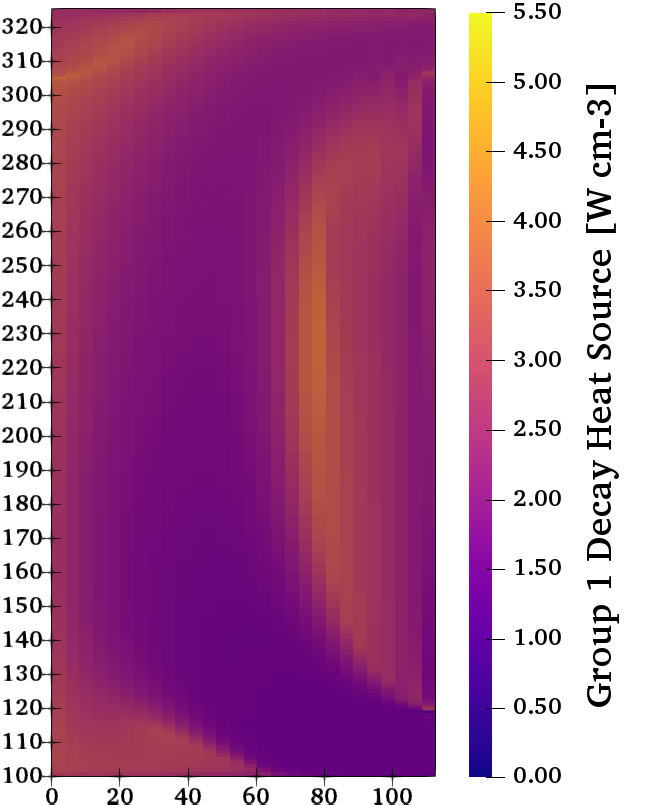
\includegraphics[width=\textwidth]{heat1-plasma}
    \end{subfigure}
    \begin{subfigure}[t]{.325\textwidth}
        \centering
        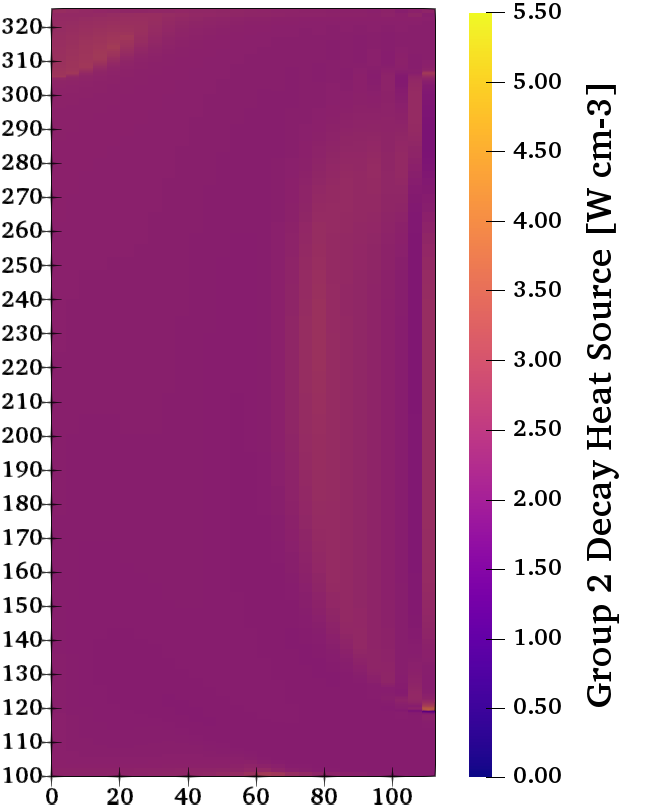
\includegraphics[width=\textwidth]{heat2-plasma}
    \end{subfigure}
    \begin{subfigure}[t]{.325\textwidth}
        \centering
        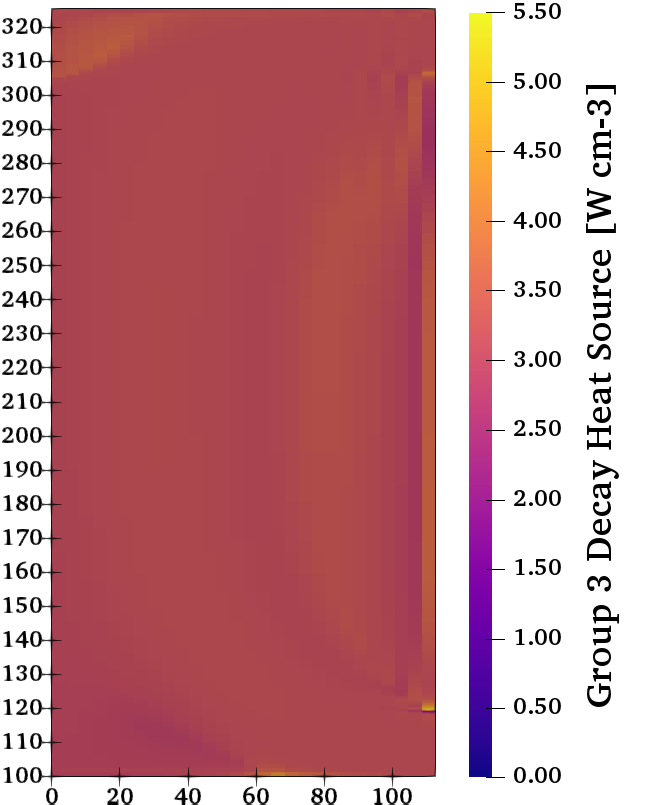
\includegraphics[width=\textwidth]{heat3-plasma}
    \end{subfigure}
    \caption{Decay heat source distribution in the core for decay heat groups
    1 to 3 (from left to right). Refer to Figure \ref{fig:decayheattemp} for
    the height and radius scales on the y and x axes, respectively. Note the
    different scales for each distribution.}
    \label{fig:decayheat}
\end{figure}

Figure \ref{fig:decayheat} shows the decay heat source distribution in the
core for groups 1 to 3. Readers may refer to Table
\ref{table:decayheat} for the associated decay time constants.
Similar to the delayed neutron precursor distributions, the shorter-lived
decay heat precursors show greater build-up in the recirculation zones
compared with the longer-lived decay heat precursors that are more evenly
distributed throughout the core.

Figure \ref{fig:decayheattemp} shows the
difference in core temperatures at steady state with decay heat modeling
relative to the core temperatures without decay heat in Figure
\ref{fig:flow-temp}. This figure uses a different color map to clearly
distinguish between positive and negative temperature differences in the core.
The hotspots in the recirculation zones are approximately
2 to 4 K cooler, while the cooled salt flowing in from the inlet is
approximately 2 K hotter. These regions correspond to the hottest and coldest
areas in the core and the results agree with the expectation that the extreme
temperatures would be affected the most by the introduction of decay heat
precursors. The difference between the outlet and inlet temperatures falls
from 101.1 K to 98.9 K as some of the decay heat precursors deposit heat in
the outer loop region. The figure also shows some nonphysical oscillations in
the temperature near the outlet because the mesh near the boundary is too
coarse for the given outlet velocities. Users can avoid these oscillations
near the outlet by using a mesh
that is progressively finer towards the boundary. The
present author could not resolve this issue due to time constraints.

\begin{figure}[htbp!]
    \centering
    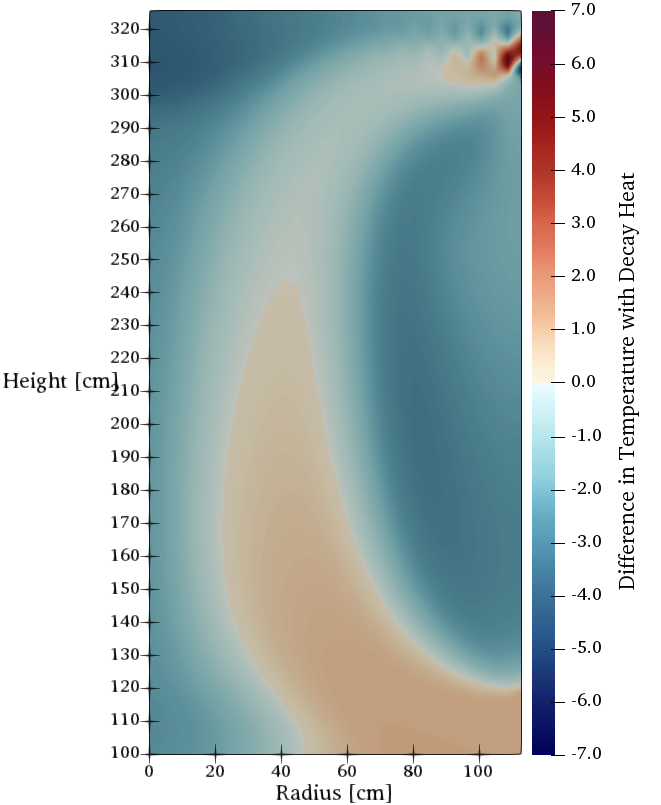
\includegraphics[width=.55\textwidth]{decay-heat-temp}
    \caption{Difference in core temperatures at steady state with decay heat
    relative to the result without decay heat (Figure \ref{fig:flow-temp}).}
    \label{fig:decayheattemp}
\end{figure}
